

\documentclass[11pt,english,ngerman, headsepline]{scrreprt}
\usepackage{lmodern}
\renewcommand{\sfdefault}{lmss}
\renewcommand{\ttdefault}{lmtt}
\usepackage[T1]{fontenc}

\usepackage{listings}

\usepackage[utf8]{inputenc} \usepackage[a4paper]{geometry}
\geometry{verbose,tmargin=3cm,bmargin=3cm,lmargin=3cm,rmargin=2.75cm,headheight=1cm,headsep=0.666cm,footskip=1cm}
\setcounter{secnumdepth}{3}
\setcounter{tocdepth}{3}
\setlength{\parskip}{\medskipamount}
\setlength{\parindent}{0pt}
\usepackage{babel}

\usepackage{verbatim} 
\usepackage{float}  
\usepackage{url}
\usepackage{graphicx}
\usepackage{setspace}
\usepackage[square,sort,numbers]{natbib}
\usepackage[utf8]{inputenc}
\usepackage{graphicx}
\usepackage[xindy,toc]{glossaries}



\setstretch{1.4}
\usepackage[usenames,dvipsnames]{color}
\usepackage[unicode=true, 
 bookmarks=true,bookmarksnumbered=false,bookmarksopen=true,bookmarksopenlevel=2,
 breaklinks=false,pdfborder={0 0 0},backref=false,colorlinks=false]
 {hyperref}
\hypersetup{pdftitle={Vergleich und Evaluation zwischen modernen und traditionellen Datenbankkonzepten 
unter den Gesichtspunkten Skalierung, Abfragem�glichkeit und Konsistenz.},
 pdfauthor={Nils M. Petersohn}}
 
\makeatletter

%%%%%%%%%%%%%%%%%%%%%%%%%%%%%% LyX specific LaTeX commands.
\providecommand{\LyX}{L\kern-.1667em\lower.25em\hbox{Y}\kern-.125emX\@}
%% Because html converters don't know tabularnewline
\providecommand{\tabularnewline}{\\}

%%%%%%%%%%%%%%%%%%%%%%%%%%%%%% Textclass specific LaTeX commands.
\newenvironment{lyxcode}
{\par\begin{list}{}{
\setlength{\rightmargin}{\leftmargin}
\setlength{\listparindent}{0pt}% needed for AMS classes
\raggedright
\setlength{\itemsep}{0pt}
\setlength{\parsep}{0pt}
\normalfont\ttfamily}%
 \item[]}
{\end{list}}

%%%%%%%%%%%%%%%%%%%%%%%%%%%%%% User specified LaTeX commands.
%% Flexibles Seitenlayout
\usepackage[automark]{scrpage2}

%% Mehrspaltenlayout ermöglichen
\usepackage{multicol}

%% Unterst\"utzung f\"ur Farben
\usepackage{color}

%% Schönere Tabellen
\usepackage{booktabs, longtable}

%% Schönerer Blocksatz
\usepackage{microtype}
%% Mehr Platz zwischen Überschrift und Tabelle
\newcommand{\@ldtable}{}
\let\@ldtable\table
\renewcommand{\table}{ %
    \setlength{\@tempdima}{\abovecaptionskip} %
    \setlength{\abovecaptionskip}{\belowcaptionskip} %
    \setlength{\belowcaptionskip}{\@tempdima} %
    \@ldtable %
}

%% Verschiedene Symbole und Zeichen wie (c), ¤
\usepackage{textcomp}

%% Fehlerkorrektur f\"ur Marginalien
\usepackage{fixltx2e }%,mparhack

%% Deutsche Kurzfassung und englisches Abstract auf eine Seite
\renewenvironment{abstract}{
    \@beginparpenalty\@lowpenalty
        \begin{center}
            \normalfont\sectfont\nobreak\abstractname
        \end{center}
    \@endparpenalty\@M
}{
    \par
}

%% Alle Seiten vor dem Inhaltsverzeichnis sind römisch nummeriert
\pagenumbering{roman}
\let\myTOC\tableofcontents
\renewcommand\tableofcontents{
    \begin{spacing}{1.1}
    \myTOC
    \end{spacing}
    \clearpage
    \pagenumbering{arabic}
}

%% Kopfzeile um Logo erg\"anzen
\clearscrheadfoot
\ohead{\\\headmark}
\ihead{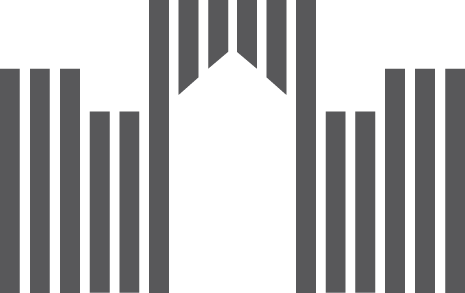
\includegraphics[scale=0.25]{pics/FH-Logo-only-gray}}%\pagemark}
\ofoot[\pagemark]{\pagemark}

%% Randnotizen anpassen
\setlength{\marginparwidth}{22mm}
\let \oldmarginpar = \marginpar
\renewcommand{\marginpar}[1]{%
    \-\oldmarginpar[\raggedleft\footnotesize\sf #1]%
        {\raggedright\footnotesize\sf #1%
    }}

%% Zitate am Kapitelanfang
%\usepackage{epigraph}
%\setlength{\epigraphwidth}{9cm}

%% Code-Block-Formatierung
\lstdefinestyle{default}{ %
    backgroundcolor={\color[rgb]{0.95,0.95,0.95}}, %
    basicstyle={\small\ttfamily}, %
    breaklines=true, %
    frame=l, %
    language={[Sharp]C}, %
    lineskip=-0.1pt, %
    numbers=left, %
    rulecolor={\color[rgb]{0.5,0.5,0.5}}, %
    xleftmargin={0.75cm}, %
    xrightmargin={0cm} %
}
\lstdefinelanguage{JavaScript} {
	morekeywords={
		break,const,continue,delete,do,while,export,for,in,function,
		if,else,import,in,instanceOf,label,let,new,return,switch,this,
		throw,try,catch,typeof,var,void,with,yield
	},
	sensitive=false,
	morecomment=[l]{//},
	morecomment=[s]{/*}{*/},
	morestring=[b]",
	morestring=[d]'
}

\lstset{
	frame=tb,
	framesep=5pt,
	basicstyle=\footnotesize\ttfamily,
	showstringspaces=false,
	keywordstyle=\ttfamily\bfseries\color{CadetBlue},
	identifierstyle=\ttfamily,
	stringstyle=\ttfamily\color{OliveGreen},
	commentstyle=\color{GrayBlue},
	rulecolor=\color{Gray},
	xleftmargin=5pt,
	xrightmargin=5pt,
	aboveskip=\bigskipamount,
	belowskip=\bigskipamount
}
\makeatother

\setlength{\parindent}{5pt} 
\setlength{\parskip}{1ex}

\parindent 0pt


\begin{document}


\titlepage

\begin{center}

\includegraphics[width=5cm]{pics/FH-Logo}\vspace{0.5cm}

\par\end{center}

\noindent \begin{center}
\textsf{\textbf{\Large University of Applied Sciences}}\\
\textsf{\large Department of Informatics and Media}\\
\vspace{1cm}

\par\end{center}

\noindent \begin{center}
\textsf{\textbf{\huge Apache Camel  \\ Example Application -
Earthquake Mashup}}\textsf{}\\ \textsf{}\\
\textsf{\Large Systemintegration 1. Term Master Informatik \\ Prof.
Dr. Preuss }


\par\end{center}{\Large \par}

\vspace{2cm}


\noindent \begin{center}
{\huge }\begin{tabular}{rl}
Provided by: & Robert Stümer, Nils Petersohn, Steffen
Reinkensmeier\tabularnewline & 27.01.2011.\tabularnewline
\end{tabular}
\par\end{center}{\huge \par}

\vspace{1cm}




\noindent \begin{center}
\medskip{}
\begin{tabular}{rl}
\tabularnewline
\end{tabular}
\par\end{center}

\newpage{}

%
\begin{comment}
leere Seite nach dem Titelblatt

dann Aufgabenstellung
\end{comment}


\begin{comment}
%\pagestyle{scrheadings}    %Kopfzeile ein

\noindent \begin{center}
\textsf{\textbf{\large Selbstst\"andigkeitserkl\"arung}}
\par\end{center}{\large \par}

\noindent Hiermit erkl\"are ich, dass ich die vorliegende Arbeit zum
Thema

\smallskip{}


\noindent \begin{center}
\textsf{Medienverwaltung mit Eclipse und Equinox}
\par\end{center}

\smallskip{}


\noindent vollkommen selbstst\"andig verfasst und keine anderen als
die angegebenen Quellen und Hilfsmittel benutzt sowie Zitate kenntlich
gemacht habe. Die Arbeit wurde in dieser oder \"ahnlicher Form noch
keiner anderen Pr\"ufungsbeh\"orde vorgelegt.

\medskip{}


\noindent Brandenburg/Havel, den dd.MM.yyyy

\vspace{1.7cm}


\noindent Unterschrift 

\selectlanguage{ngerman}
\end{comment}
%\newpage{}

%\noindent \begin{center}
%\textsf{\textbf{\large Danksagung}}
%\par\end{center}{\large \par}


%\newpage{}
%\begin{abstract}

%\end{abstract}

%\selectlanguage{english}%
%\begin{abstract}
%This is a second abstract in english.

%\newpage{}
%\end{abstract}

\selectlanguage{ngerman}%
\tableofcontents{}

\pagestyle{scrheadings}    %Kopfzeile ein


%==========================================================================
% DOCUMENT START 
%==========================================================================

\chapter{Introduction / Motivation / Project}
 
 Systemintegration is the part of a software architectur. It helps to connect
 components or subsystems together. Certain patterns are used in the industry
 today. Using and learning EIP (``Enterprise Integration Pattterns'') with
 Apache Camel is the goal of this Project.\\
 
 The Example for this project is all about earthquake data from around the
 world. The Application is able to read earthquake data from various rss Feeds
 and processes it. During the processing the data will be in form of XML and
 Java Objects. The data will be enriched, splitted, sorted, aggregated,
 normalized, marshalled umarshalled and finally provided again in form of a
 restful service.\\
 
 The specified task is as follows:
 
 \begin{enumerate}
   
 
 \item Read Earthquake Data continously from those two RSS Streams
 \begin{itemize}
  	\item \url{http://geofon.gfz-potsdam.de/db/eqinfo.php?fmt=rss}
  	\item \url{http://earthquake.usgs.gov/eqcenter/catalogs/eqs1day-M2.5.xml}
  \end{itemize}
  \item enrich this data with other related information like the weather in this
  area at this time. Data can be from here: \url{http://www.programmableweb.com}.
  \item sort the earthquakes by the earthparts where they appear
  \item if the earthquake has a strength of more than ``M 5.5'' than send an
  formated warning email to an email adress.
  \item  provide this data via a Restful interface in form of a list of the
  earthparts with an xlink to detailed information of the earthquakes.
  
 \end{enumerate}

\chapter{Information Collection and Normalization}\label{chapter:normalization}

The Normalizer \cite{hohpe2003enterprise} (Pic. \ref{normalizerPic}) routes each
message type through a custom Message Translator so that the resulting messages match a common format. 
The different message formates are collected in one channel
(``$direct:collectorChannel$'') and than routed according to their xml format.
The Routing is accomlished with a xpath condition which routes the messages to
the specified Message Translators \cite{hohpe2003enterprise} (Pic.
\ref{translatorPic}). Here The Translator is implemented with a XSLT formatter
\url{http://www.w3.org/TR/xslt}.
The relative source code is listed in \ref{normalizerTranslator.java}


  \begin{figure}[h!]
	\begin{center}
	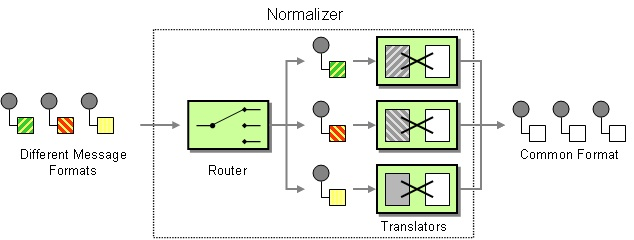
\includegraphics[width=0.9\textwidth]{pics/NormalizerDetail.jpg}
	\end{center}
	\caption{Normalizer Pattern \cite{hohpe2003enterprise}}
	\label{normalizerPic} 
   \end{figure}
   
   
   \begin{figure}[h!]
	\begin{center}
	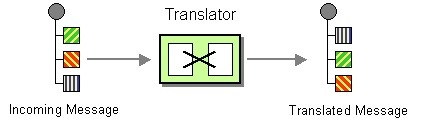
\includegraphics[width=0.9\textwidth]{pics/MessageTranslator.jpg}
	\end{center}
	\caption{Translator Pattern \cite{hohpe2003enterprise}}
	\label{translatorPic} 
   \end{figure}



\lstinputlisting[caption={Normalizer and Translator Source Code},
label={normalizerTranslator.java},style=default]{code/normalizerTranslator.java}




\chapter{Aggregating Information Sources} 



\begin{quote}
``The Aggregator is a special filter that recieves a strem of messages an
didentifies messages that are correlated. Once a complete set of messages has
been recied, the Aggregator collects information from each correlated message
and publishes a single, aggregated message to the output channel for further
processing.'' \cite{hohpe2003enterprise}
\end{quote}

  \begin{figure}[h!]
	\begin{center}
	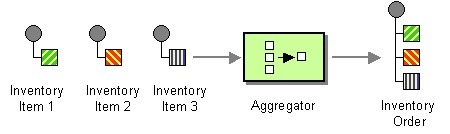
\includegraphics[width=0.9\textwidth]{pics/Aggregator.jpg}
	\end{center}
	\caption{Aggregator Pattern \cite{hohpe2003enterprise}}
	\label{utilityTree} 
   \end{figure}


Camel provides a method named $aggregate$ with two parameters, first the
identifier (the message header which was defined before in chapter
\ref{chapter:normalization}) of the messages to aggregate  and second the
strategy (as a Object: $SpecialAggregationStrategy$ which implements\\
$org.apache.camel.processor.aggregate.AggregationStrategy$). Code listing
\ref{aggregateinputstreams.java} shows the implementation in this project for
the normalized messages from Chapter \ref{chapter:normalization}. Code listing
\ref{aggregationstrategy.java} shows the strategy which is fairly simple.


\lstinputlisting[caption={Aggregator},
label={aggregateinputstreams.java},style=default]{code/aggregateinputstreams.java}


\lstinputlisting[caption={Aggregation Strategy},
label={aggregationstrategy.java},style=default]{code/aggregationstrategy.java}


\chapter{Enrich Data with related Information}
Information can be
added to the original Message with the Message Transformation Pattern ``Content
Enricher'' .

  \begin{figure}[h!]
	\begin{center}
	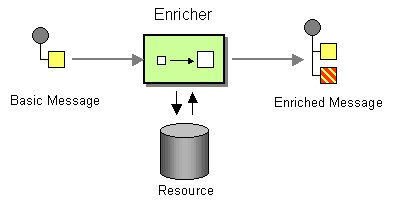
\includegraphics[width=0.7\textwidth]{pics/DataEnricher.jpg}
	\end{center}
	\caption{Content Enricher Pattern \cite{hohpe2003enterprise}}
	\label{contentEnricherPic} 
   \end{figure}

``The Content Enricher (Pic. \ref{contentEnricherPic}) uses information inside
the incoming message to retrieve data from an external
source.\cite{hohpe2003enterprise}''
This is accomplished via the coordinates of the earthquake. which are used to
retrieve area information \\
\url{http://api.wunderground.com/auto/wui/geo/GeoLookupXML} \\and weather
information from \url{http://www.worldweatheronline.com/feed/weather.ashx}.
See Listing \ref{enricherCode} for the source code.

\lstinputlisting[caption={Enricher},
label={enricherCode},style=default]{code/enricher.java}

The $EnrichmentProcessor$ can now work with the java instances see Listing
\ref{conricherProcessor.java}

\lstinputlisting[caption={EnrichmentProcessor},
label={conricherProcessor.java},style=default]{code/conricherProcessor.java}





For the most flexibility the XML Message is automatically unmarshalled to the
specified Java objects via the JAXB Umarshaller. 

\begin{itemize}
  \item Earthpart
  \item EarthPartCollection
  \item EarthquakeCollection
  \item Earthquake
  \item EintragCollection
  \item Weather
  \item WeatherWrapper
\end{itemize}

This is easyliy accomplished with jaxb Annotations in the data models. For more
information on JAXB please visit: \\
\url{http://www.oracle.com/technetwork/articles/javase/index-140168.html}

In Camel, data formats are pluggable transformers that can transform messages
from one form to another and vice versa. Each data format is represented in
Camel as an interface in org.apace.camel.spi.DataFormat containing two methods:
\begin{itemize}
  \item marshal—For marshaling a message into another form, such as
marshaling Java objects to XML, CSV, EDI, HL7, or other well-known data
models.
\item unmarshal—The reverse operation which turns data from well known 
formats back into a message.
\end{itemize}
You may already have realized that these two functions are
opposites, meaning that one is capable of reversing what the other has done, as illustrated in
figure \ref{picMarshalling}. \cite{ibsen2010camel}



  \begin{figure}[h!]
	\begin{center}
	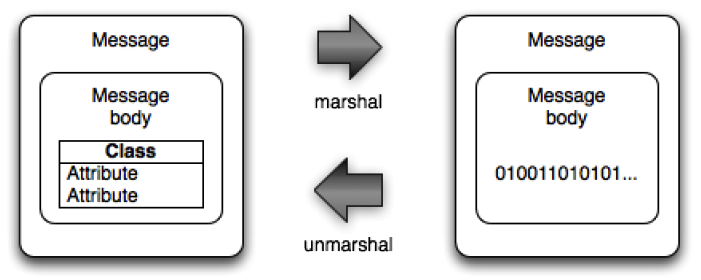
\includegraphics[width=0.7\textwidth]{pics/marshalling}
	\end{center}
	\caption{Transforming with Data Formats \cite{hohpe2003enterprise}}
	\label{picMarshalling} 
   \end{figure}

The Marshalled State is shown in the Class Diagram (Pic \ref{modelDia.JPG}) for
the package\\ $edu.fhb.sysint.camel.model$\\
The marshalled state is the XML Form (Pic. \ref{picmarshalledEarthparts},
\ref{picmarshalledEarthquake.png})

 \begin{figure}[h!]
	\begin{center}
	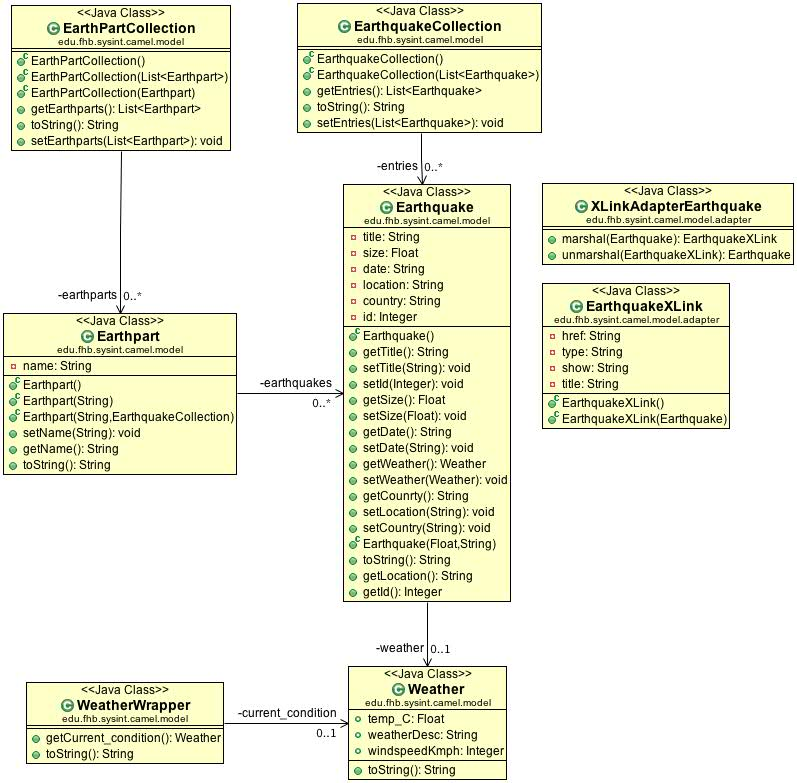
\includegraphics[width=0.99\textwidth]{pics/modelDia.JPG}
	\end{center}
	\caption{edu.fhb.sysint.camel.model Package}
	\label{modelDia.JPG} 
   \end{figure}
   
   
   \begin{figure}[h!]
	\begin{center}
	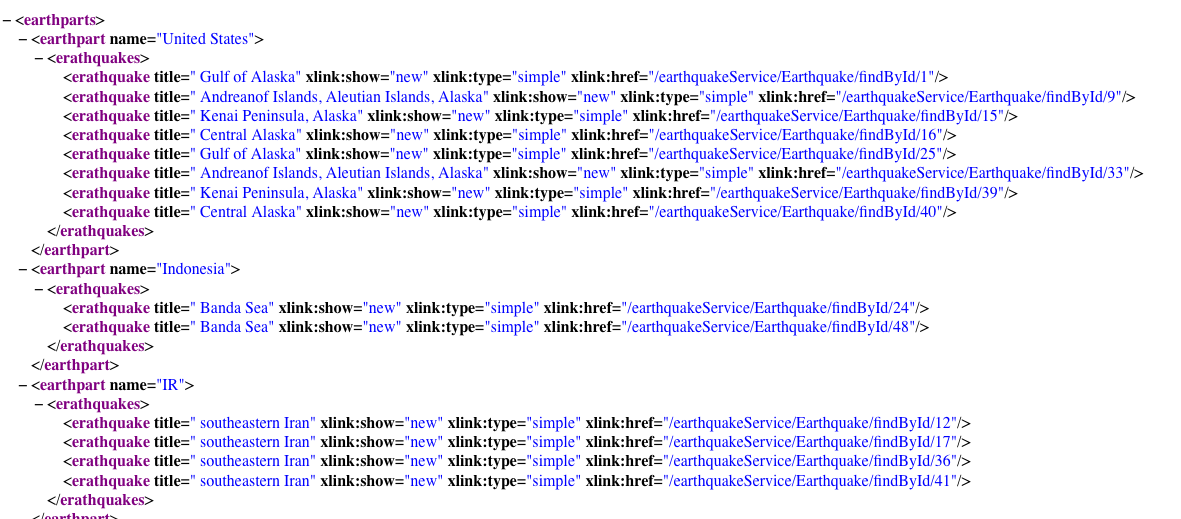
\includegraphics[width=0.99\textwidth]{pics/marshalledEarthparts}
	\end{center}
	\caption{marshalled Earthparts}
	\label{picmarshalledEarthparts} 
   \end{figure}
   
   
   \begin{figure}[h!]
	\begin{center}
	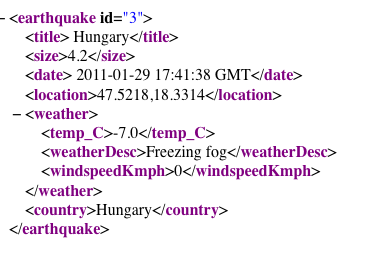
\includegraphics[width=0.7\textwidth]{pics/marshalledEarthquake}
	\end{center}
	\caption{marshalled Earthquake}
	\label{picmarshalledEarthquake.png} 
   \end{figure}



\chapter{Email Notification}

If the strength of the Earthquakes are more than M 5.5 than an email
notification must be delivered. This is implemented with Apache Camel throught
the splitter Pattern (Pic \ref{splitter}) 


 \begin{figure}[h!]
	\begin{center}
	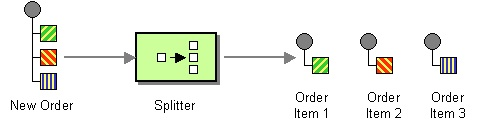
\includegraphics[width=0.7\textwidth]{pics/Sequencer.jpg}
	\end{center}
	\caption{Sequencer with Splitter Pattern}
	\label{splitter} 
   \end{figure}


The Source is splitted and aggregated. If The xPath evaluates to true the
message is reformated in a human readable format and sent to the provided email
address.

\lstinputlisting[caption={Splitting Pattern},
label={splitting.java},style=default]{code/splitting.java}


The Resulting Email is shown in Pic \ref{EmailResult}


 \begin{figure}[h!]
	\begin{center}
	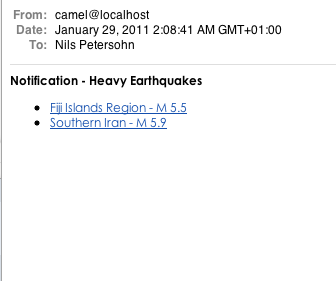
\includegraphics[width=0.8\textwidth]{pics/EmailResult.jpg}
	\end{center}
	\caption{Email Result}
	\label{EmailResult} 
   \end{figure}

 




\chapter{RESTful Service}

The Mashup is provided via a REST Web Service
(\url{http://localhost:9000/earthquakeService/})
The provided Data is sorted by Earthparts which were determined via the
enrichment Phase.
Camel has the availability to establish a REST Service with the Help of the
Apache CXF Project which works closly JAXB (marshalling/umarshalling). 
The Rest Router (Listing \ref{rest.java} ) determines the requested URL and
requests the DAO Layer \cite{fowler2002patterns} to send the correct response
Data.

\lstinputlisting[caption={Rest Router}, 
label={rest.java},style=default]{code/rest.java}

The CXF Endpoint is configured with the Definition class (Listing
\ref{cxf.java})
   
\lstinputlisting[caption={CXF Service Definition},
label={cxf.java},style=default]{code/cxf.java}

\chapter{XLink with jaxb Adapters}
Jaxb allows the use of the Adapter Pattern \ref{gamma1995design}. This allows to
define special Marshalling for Objects.
When the jaxb umarshaller gets to the Earthpart Object than the data field
``Earthquakes'' is not umarshalled normally. 
The Annotation @XmlJavaTypeAdapter (Listing \ref{earthpartCode.java}) Redirects that
action to special marshalling/umarshalling methods. 

\lstinputlisting[caption={Earthpart Class},
label={earthpartCode.java},style=default]{code/earthpartCode.java}

Since the Classes for marshalling this special requirement are located in an
extra package $edu.fhb.sysint.camel.model.adapter$ it was possible to use the
namespace mechanism at package level. 


``Annotations that can be applied to the
package element are referred to as package-level annotations. An annotation with
ElementType.PACKAGE as one of its targets is a package-level annotation.
Package-level annotations are placed in a package-info.java
\ref{package-info.java} file. This file should contain only the package statement, preceded by annotations. When the
compiler encounters package-info.java file, it will create a synthetic
interface, package-name.package-info. The interface is called synthetic because
it is introduced by the compiler and does not have a corresponding construct in
the source code. This synthetic interface makes it possible to access
package-level annotations at runtime.\cite{packageinfo}''




\lstinputlisting[caption={package-info.java for the Adapter Package},
label={package-info.java},style=default]{code/package-info.java}




\chapter{Deployment Steps}
The System is deployed via the Apache Servicemix OSGI Runtime Container.
``Apache ServiceMix is an open source ESB (Enterprise Service Bus) that combines
 the functionality of a Service Oriented Architecture (SOA) and an Event Driven
 Architecture (EDA)  to create an agile, enterprise ESB.\cite{sm} ''
 
The Camel Version used is ``2.4.0-fuse-02-00'' from the repository
``\url{http://repo.fusesource.com/maven2/}''.

\begin{enumerate}
  
\item  download fuse 4-3-0 file and unpack to ~/downloadedFuse
\url{http://fusesource.com/product_download/fuse-esb-apache-servicemix/4-3-0-fuse-03-00/unix}

\item  replace ~/downloadedFuse/etc/org.apache.karaf.features.cfg key value pair "featuresBoot=..." with

featuresBoot=config,activemq-broker,camel,camel-http,camel-jaxb,jbi-cluster,war,\\
servicemix-cxf-bc,servicemix-file,servicemix-ftp,servicemix-http,servicemix-jms,\\
servicemix-mail,servicemix-bean,servicemix-camel,servicemix-cxf-se,servicemix-drools,\\
servicemix-eip,servicemix-osworkflow,servicemix-quartz,servicemix-scripting,\\
servicemix-validation,servicemix-saxon,servicemix-wsn2005,camel,camel-spring-osgi,\\
cxf,camel-cxf,camel-jetty,web,cxf-jaxrs,camel-rss,activemq-camel,rome-osgi,camel-mail\\
  
  \item please modify the Constants in GlobalConstants.java for path settings.
  
\item  in the project root do ``mvn install''

\item start fuse with ~/downloadedFuse/bin/servicemix

\item  on the karaf shell type: ``install -s
mvn:edu.fhb.sysint.camel/ApacheCamelEarthquakeService''

\item browse to http://localhost:9000/earthquakeService/Earthparts

\end{enumerate}



%\chapter{verwendete EAI-Pattern}



 
%==========================================================================
% DOCUMENT END 
%==========================================================================

\bibliographystyle{alphadin}
\clearpage\addcontentsline{toc}{chapter}{\bibname}\bibliography{jabref}


\appendix
\renewcommand{\theequation}{A-\arabic{equation}}

\setcounter{equation}{0}  % reset counter \chapter*{Anhang}  % use *-form to




\listoffigures
\end{document}
